\documentclass{article}%

% Margins
\usepackage[top=1in, bottom=1in, left=1in, right=1in]{geometry}

% Fonts
\usepackage[T1]{fontenc}
\usepackage[utf8]{inputenc}

% Section formatting
\usepackage[center]{titlesec}

% Formatting
\usepackage{setspace}
\doublespacing
\usepackage{caption}
\hyphenation{con-sti-tu-tion-al}
\usepackage{amsmath}

% Media
\usepackage{graphicx}
\usepackage{wrapfig}
\usepackage{float}
\usepackage{booktabs}
\graphicspath{ {../figures/} }

% Table of Contents
\usepackage{tocloft}
\usepackage{etoolbox}

% List of Figures
\makeatletter
\renewcommand*\l@figure{\@dottedtocline{1}{0em}{7em}}
\makeatother

% Ensure dots in table of contents
\makeatletter
\renewcommand*\l@section{\@dottedtocline{1}{1.5em}{2.3em}}
\makeatother
% Rename table of contents
\renewcommand*\contentsname{\textbf{TABLE OF CONTENTS}}
% Rename list of figures
\renewcommand*\listfigurename{\textbf{LIST OF FIGURES}}

\begin{document}
\pagestyle{empty}
% Title
% \pagenumbering{roman}
\begin{center}
{\fontfamily{ptm}\Large\selectfont
    Novel Approach to Constructing an Ultra Low Cost Flowcell Biosensor\\
}
% 4 returns = ?? vspace
\vspace{1.7cm}
{\fontfamily{ptm}\large\selectfont
    THESIS\\
}
% 5 returns = ?? vspace
\vspace{2cm}
{\fontfamily{ptm}\large\selectfont
    Presented to the Faculty of the Department of Physics and Astronomy\\
    in Partial Fulfillment of the Major Requirements\\
    for the Degree of\\
}
% 6 returns = ?? vspace
\vspace{2.1cm}
{\fontfamily{ptm}\large\selectfont
    BACHELOR OF SCIENCE IN\\
    PHYSICS\\
}
% 6 returns = ?? vspace
\vspace{2cm}
{\fontfamily{ptm}\selectfont
    \large{Jeffery Summers}\\
}
% 6 returns = ?? vspace
\vspace{1.6cm}
{\fontfamily{ptm}\selectfont
    \large{May 2019}\\
}
% 6 returns = ?? vspace
\vspace{2cm}
{\fontfamily{ptm}\selectfont
    \copyright 2019 Middle Tennessee State University\\
    All rights reserved.\\
}
\vspace{0.2cm}
{\fontfamily{ptm}\small\selectfont
    The author hereby grants to MTSU permission to reproduce\\
    and to distribute publicly paper and electronic\\
    copies of this thesis document in whole or in part\\
    in any medium now known or hereafter created.\\
}
\end{center}
\pagenumbering{roman}

\pagebreak

% Signature page
% Number pages with lowercase roman numerals
\begin{center}
{\fontfamily{ptm}\selectfont
    Novel Approach to Constructing an Ultra Low Cost Flowcell Biosensor\\
}
% 3 returns = ?? vspace
\vspace{1.8cm}

{\fontfamily{ptm}\selectfont
Jeffery Summers
}
% 18 returns = ?? vspace
\vspace{8cm}
\end{center}
% Author signature
\begin{flushleft}
    {\fontfamily{ptm}\selectfont
    Signature of Author:\\
    }
\end{flushleft}
\vspace{0cm}
\hrule
\begin{flushright}
    {\fontfamily{ptm}\small\selectfont
    Department of Physics \& Astronomy\\
    May 2019\\
    }
\end{flushright}
\vspace{1.5cm}
% Thesis supervisor signature
\begin{flushleft}
    {\fontfamily{ptm}\selectfont
    Certified by:\\
    }
\end{flushleft}
\vspace{0cm}
\hrule
\begin{flushright}
    {\fontfamily{ptm}\small\selectfont
    Dr. William Robertson\\
    Department of Physics \& Astronomy\\
    Thesis Supervisor\\
    }
\end{flushright}
\vspace{1.5cm}
% Department chair signature
\begin{flushleft}
    {\fontfamily{ptm}\selectfont
    Accepted by:\\
    }
\end{flushleft}
\vspace{0cm}
\hrule
\begin{flushright}
    {\fontfamily{ptm}\small\selectfont
    Dr. Ronald Henderson\\
    Professor of Physics \& Astronomy\\
    Chair, Physics \& Astronomy\\
    }
\end{flushright}
\vspace{1.5cm}

\pagestyle{plain}
\pagebreak

% Abstract
\section*{ABSTRACT}
\addcontentsline{toc}{section}{\hspace{0.34in}Abstract}
\hspace{0.25in}
In this thesis we present our approach to constructing an ultra low-cost flowcell biosensor which is capable of determining changes in index of refraction on the order of $10^{-5}$. Our sensor utilizes 3D printed parts a one dimensional photonic crystal coupled to a prism rather than the traditional SPR metal film prism coupling system. By using this method we are able to bring the cost of manufacturing the sensor to around $\$100$, excluding the photonic crystals which can be fabricated commercially. The largest cost of the system is a USB camera which is used to collect data.\\
\pagebreak

% Table of Contents
\tableofcontents
\pagebreak

% List of Figures
\listoffigures
\pagebreak

% Introduction
\documentclass{report}
\usepackage[T1]{fontenc}
\usepackage{graphicx}
\usepackage[top=1in, bottom=1in, right=1in, left=1in]{geometry}
\usepackage{parskip}
\usepackage{pdfpages}

\usepackage{ragged2e}
\usepackage{mwe}

\setlength{\RaggedRightParfillskip}{.25\textwidth plus 1fil}
\setlength{\RaggedRightRightskip}{0pt plus .1\textwidth}
\setlength{\RaggedRightParindent}{4em}

\begin{document}
	\fontfamily{lmtt}\selectfont
    \RaggedRight
    \section*{Introduction}
    \vspace{-0.1cm}\hrule\vspace{0.2cm}
    \par{\indent Flowcell sensors have many applications; disease detection, refractive index measuring, and reactivity measuring to name a few. These sensors have been operating on the basis of electromagnetic surface phenomena for decades. Most flowcells on the market work by exploiting surface plasma oscillations (SPOs). These oscillations are highly sensitive to changes in the optical properties of the adjacent medium and follow from Maxwell's equations when the dielectric functions of each medium satisfies
    \[
        \frac{\epsilon_{spo}}{\epsilon_{adjacent}} < -1
    \]
		Metals like aluminum, copper, gold, and silver have negative dielectric functions at wavelengths in the red/infrared, so films of these metals are used as to generate SPOs in most flowcell sensors via a process known as Surface Plasmon Resonance (SPR). There are quite a few drawbacks for using metal films, however. Metals are highly reactive so they require regular maintenance. These films also require particular wavelengths of incident light to excite the oscillations. Rather than using metal films, one-dimensional photonic crystals, or multilayers, can be designed to exhibit the phenomenon of surface electromagnetic waves (SEWs) or Bloch surface waves (BSWs), named after the physicist Felix Bloch who was famous for working with periodic systems. These surface waves have the same practical application as SPOs. Multilayers overcome both of the shortcomings of metal films listed here. They can be designed to work for any wavelength and are typically made of nonreactive glass. In addition to these benefits, we expect that our 3-D printed and multilayer-based flowcell sensor will be more sensitive and precise with its measurements and be far cheaper to both build and maintain compared to traditional SPR sensors.}


			\par{To take measurements with our sensor we look at the reflected image of incident laser light. Our multilayer is designed to trap incident light in the last layer at a critical angle; this results in a dark band in our reflected image. A diagram of the process is shown below.}
\newline	
	\begin{figure}[h!]
		\raisebox{-0.5\height}{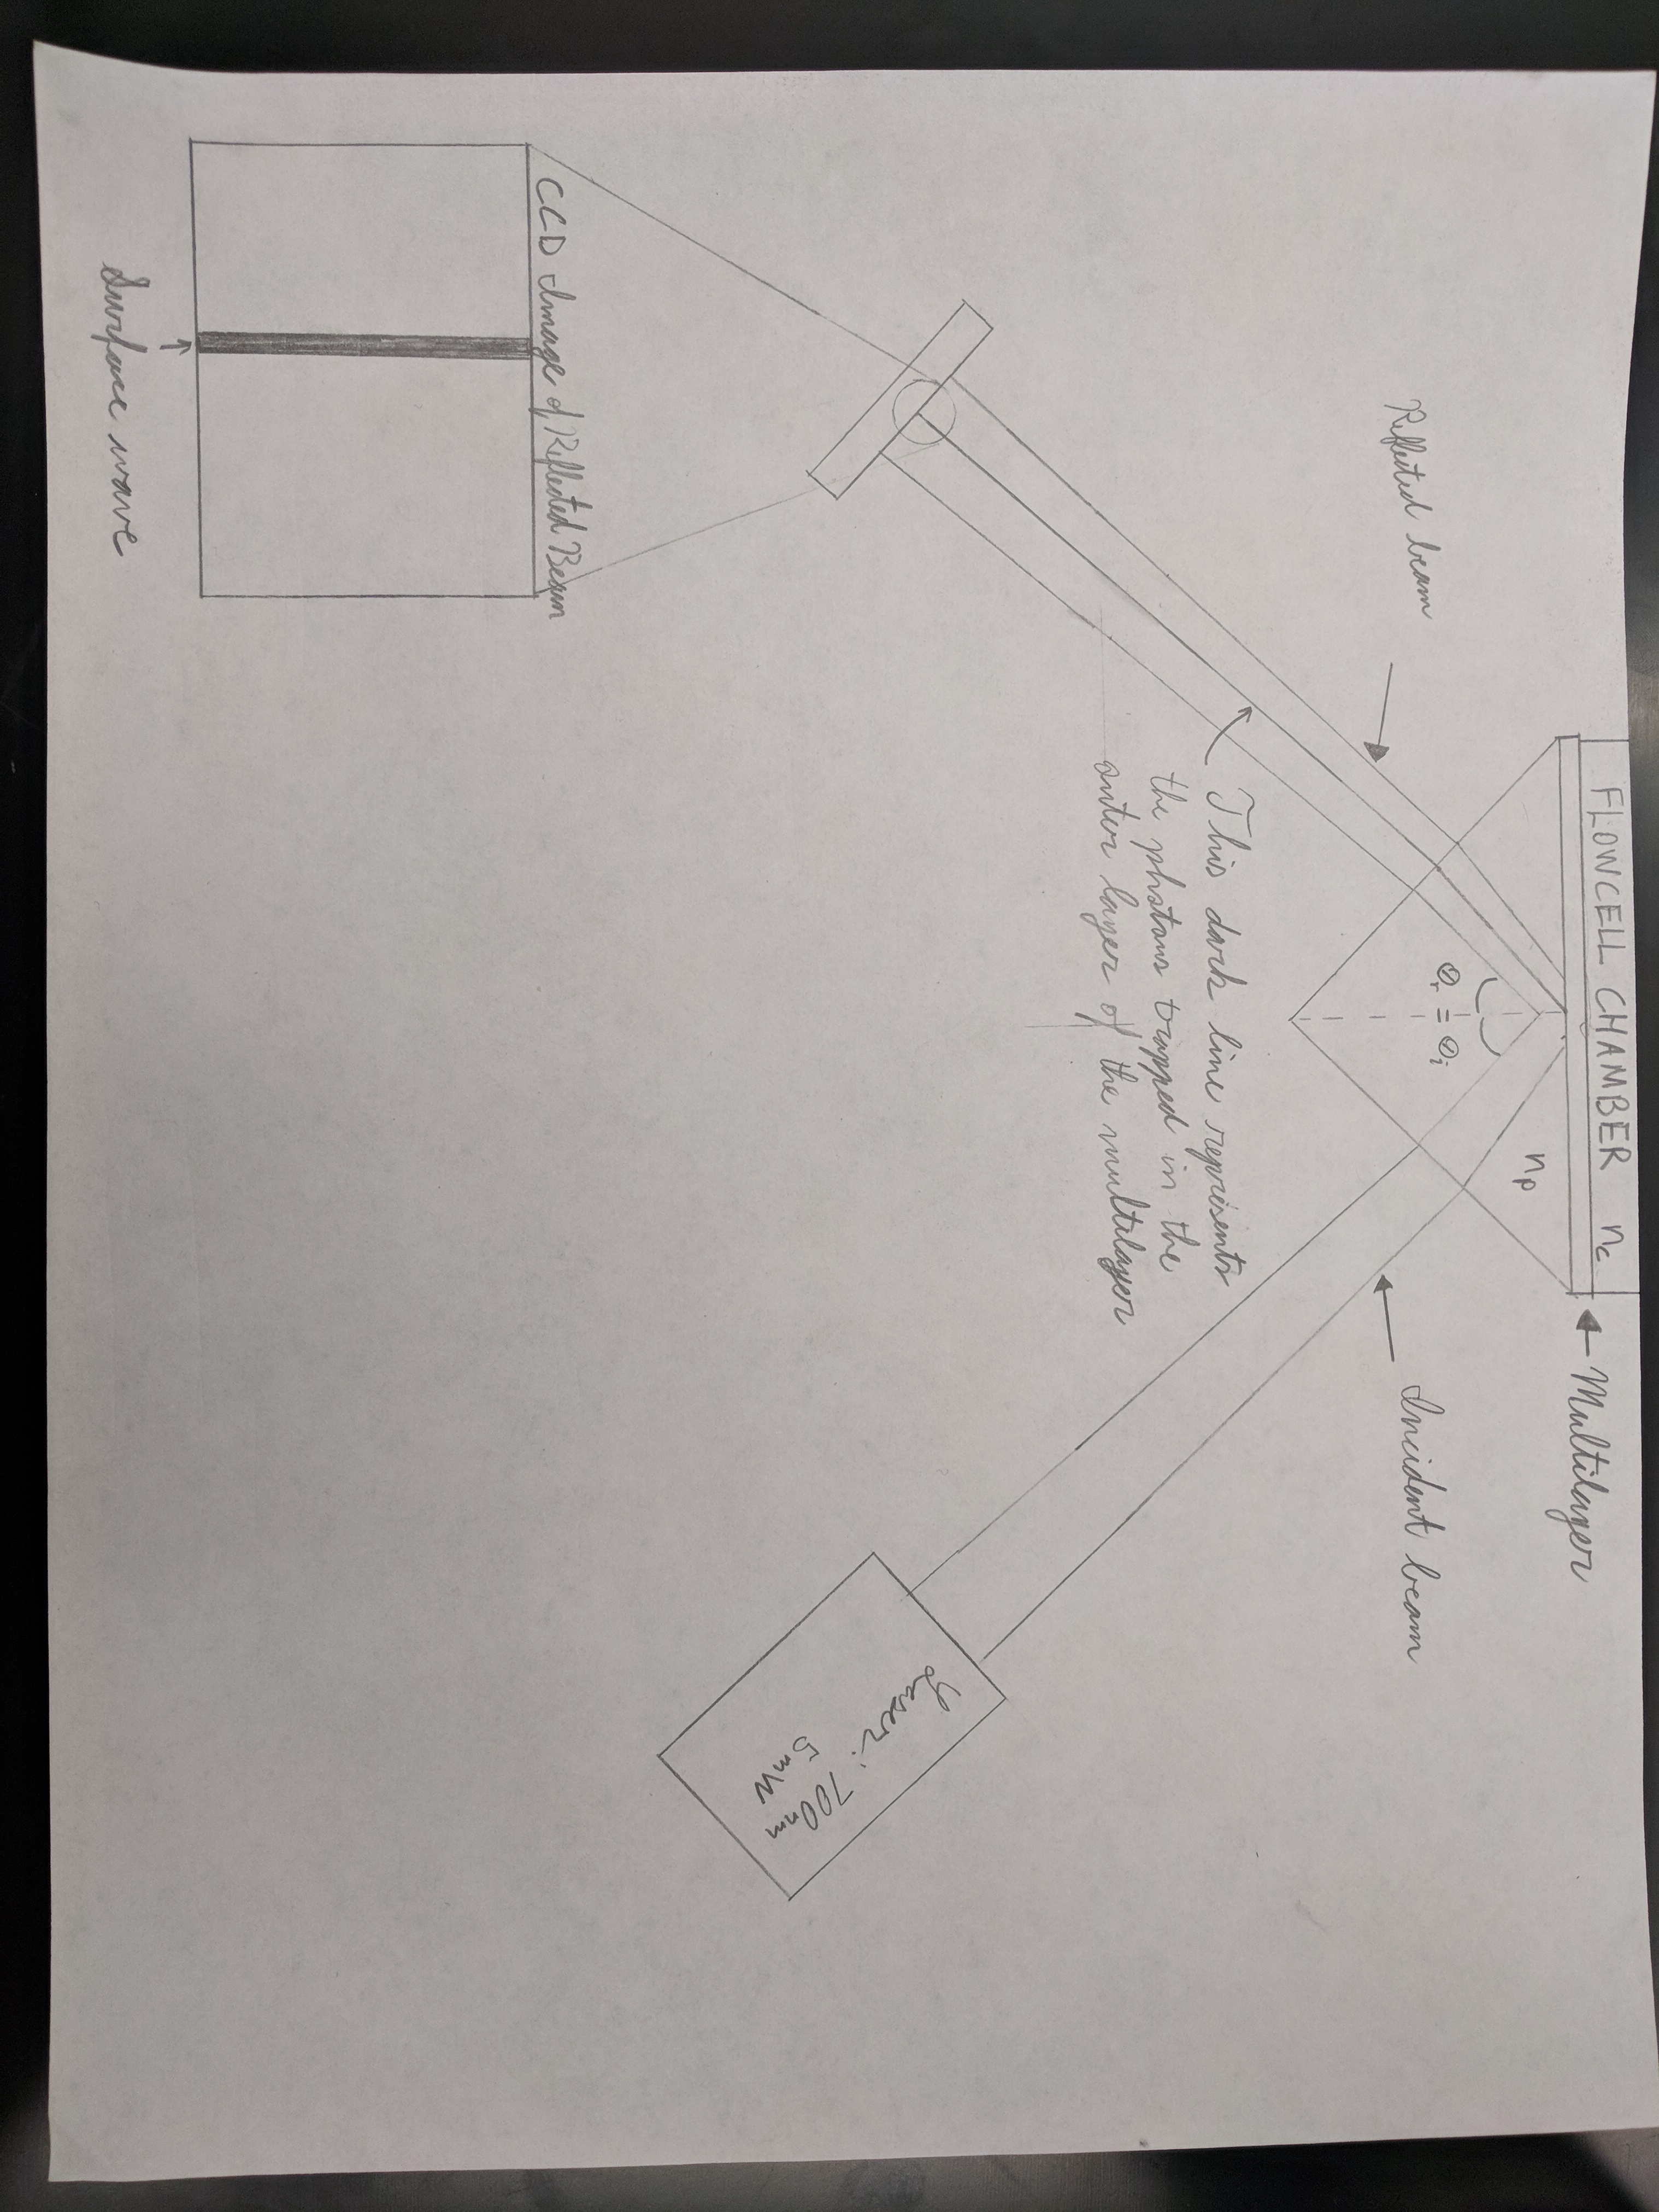
\includegraphics[height=\linewidth, angle=90, origin=c]{media/setup_diagram.jpg}}
	\end{figure}

	\par{As fluids or gases are put into the flowcell chamber the index of refraction, $n_c$, changes. The condition for total internal reflection, found from Snell's law, for the interface between a glass prism and some transmitting medium whose index of refraction varies with time is given by:}
	\[
			\sin{\theta_c} = \frac{n_t(t)}{n_g}
	\]

	\par{We obtain an expression for the angle of reflection as a function of time by the Law of Reflection:}
	\[
			\theta_r(t) = \arcsin{\frac{n_t(t)}{n_g}}
	\]


	\par{\indent Note that this expression is for a single interface and hence does not accurately reflect our setup as we have a glass prism and a multilayer. With that said, this expression for $\theta_r$ does capture the essence of our setup; the reflected angle is a function of the index of refraction of the transmission. Using this fact we can associate variations in the flowcell chamber's index of refraction with differences in the angle of reflectance. These angular differences can be calculated by tracking the variation in the position of the dark band in the reflected image.}
	\newline
	\begin{figure}[h!]
		\raisebox{-0.5\height}{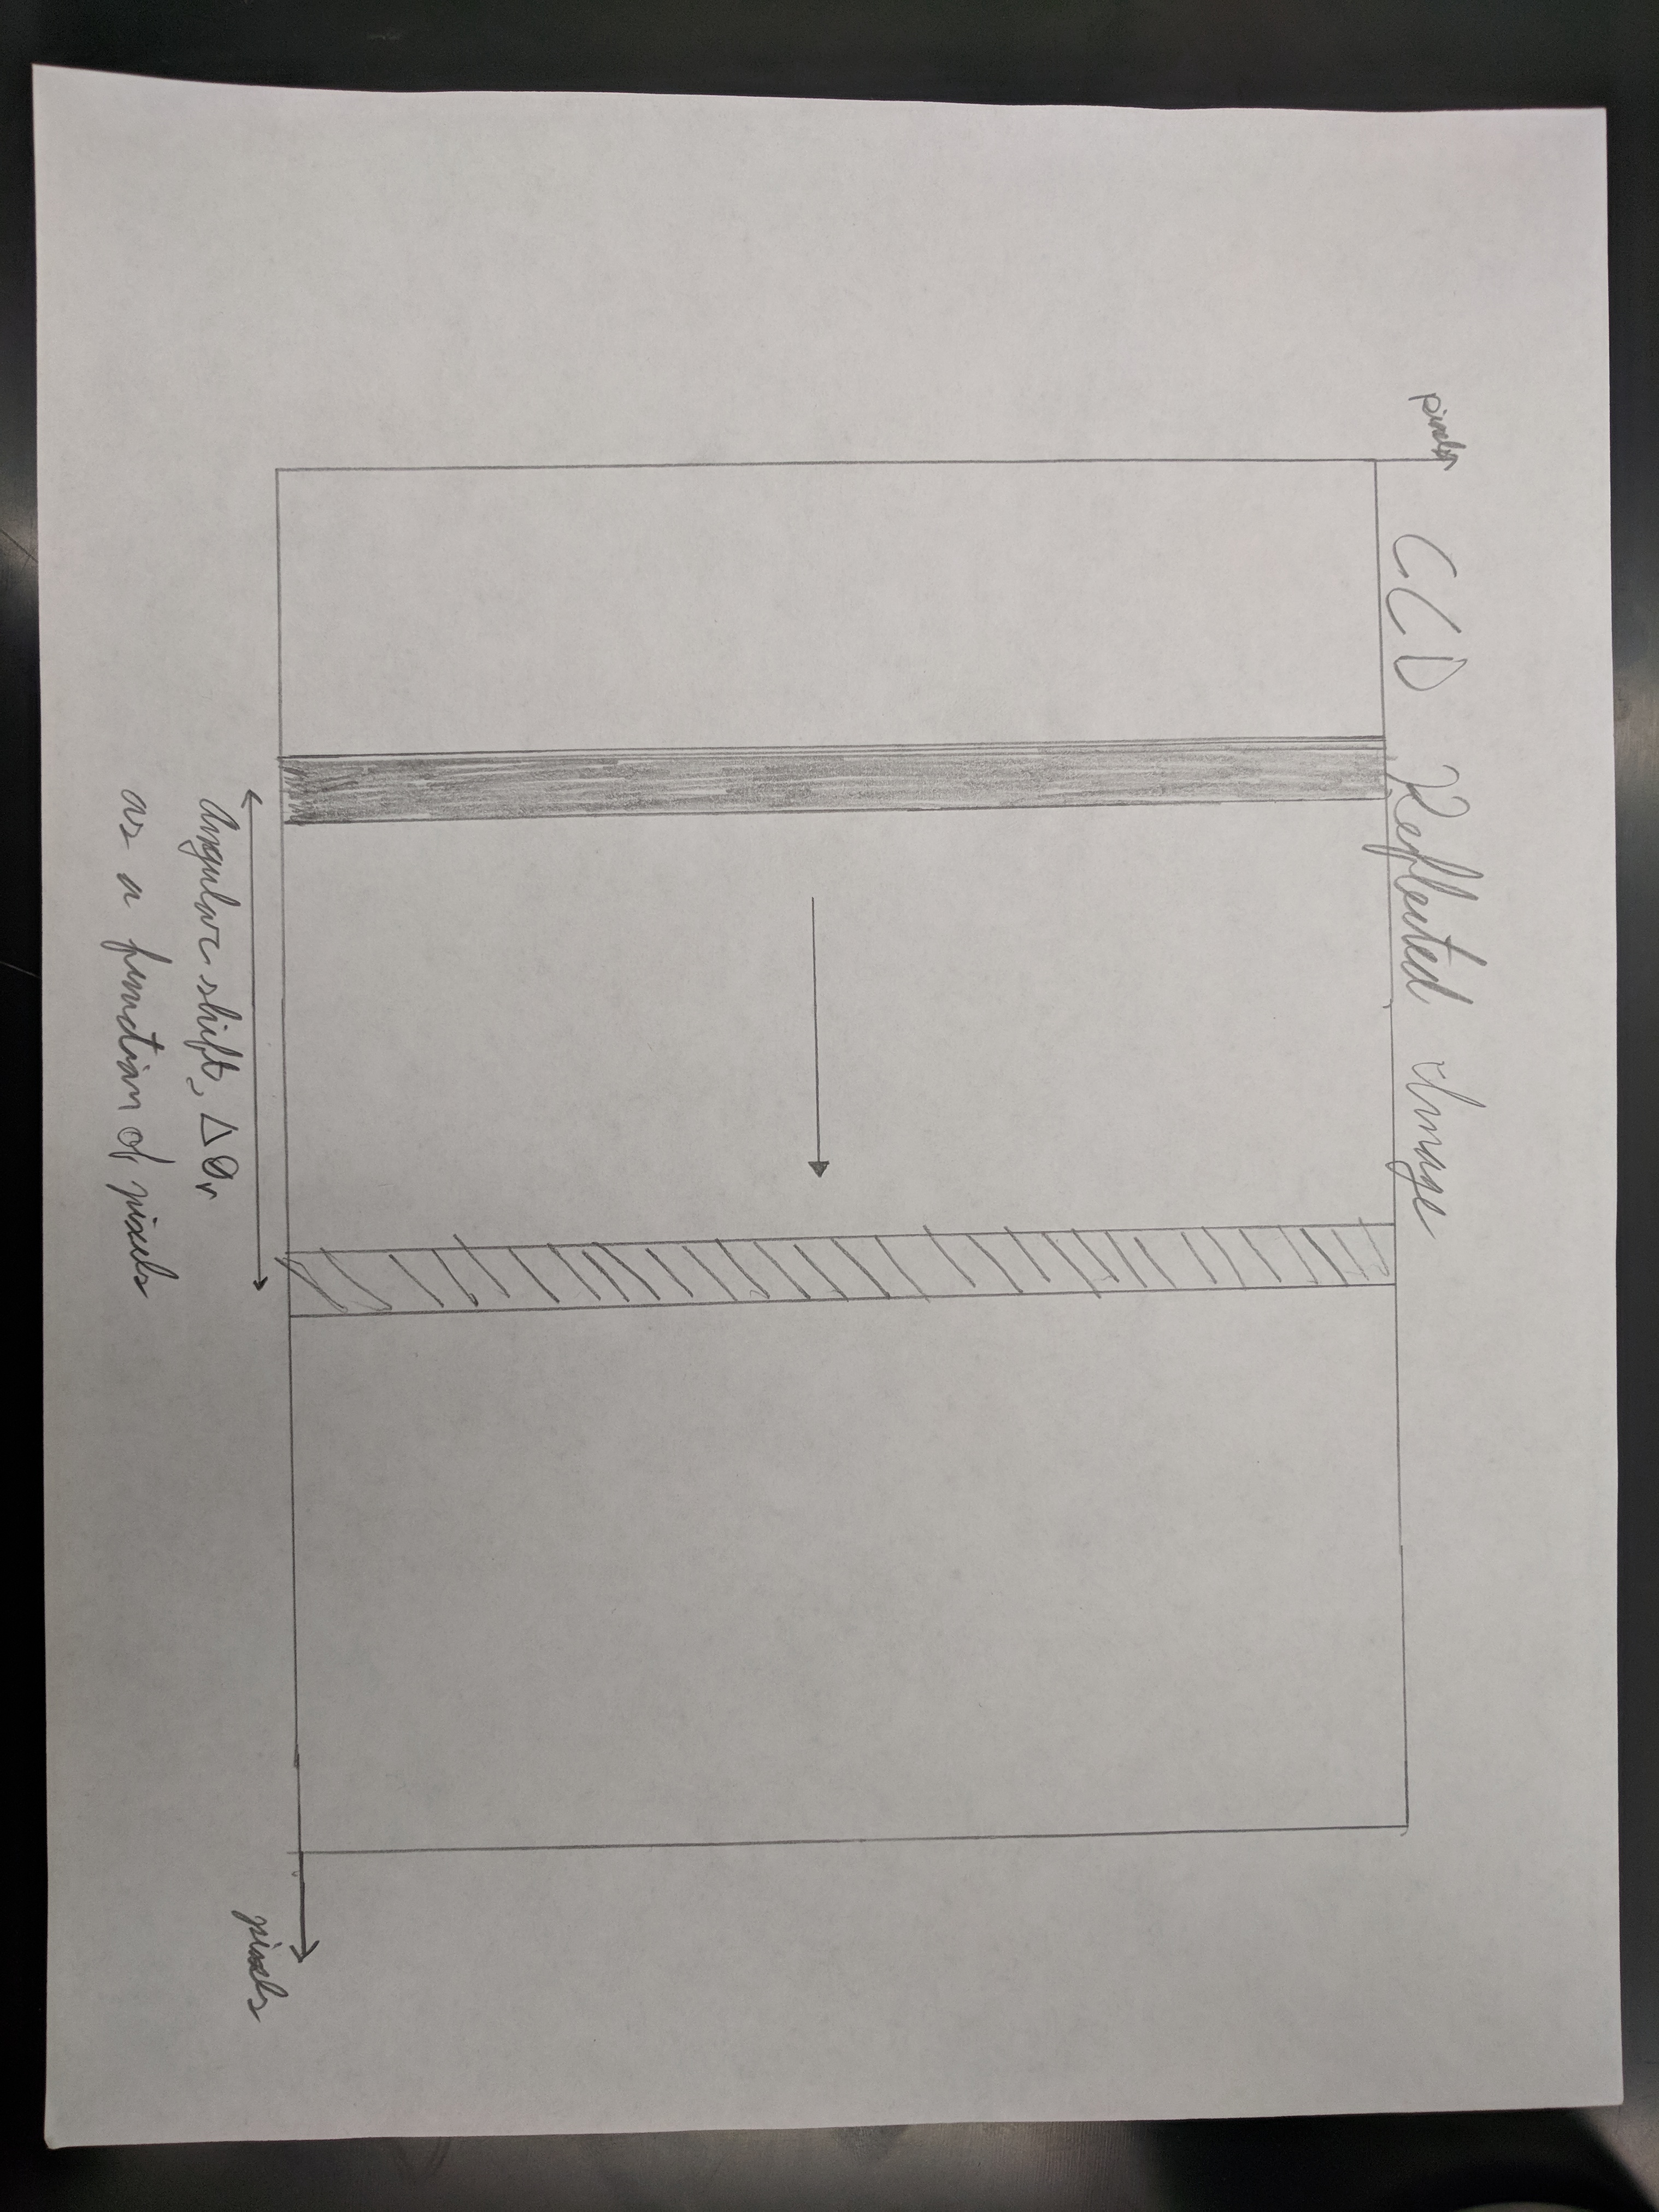
\includegraphics[height=\linewidth, angle=90, origin=c]{media/angular_sep.jpg}}
	\end{figure}
	\vspace{-3cm}
	\pagebreak
	\par{\indent Now with an an expression for the rate of change of reflected angle we can measure the index of refraction inside the flowcell chamber over time. From this data we can interpolate the mutual reactivity between molecules in a reaction, or maybe the rate of mixing of sugar water at a given temperature.

\end{document}

\pagebreak

% Experimental Setup
\section*{\textbf{II. Experimental Design}}
\addcontentsline{toc}{section}{II.\hspace{0.15in} Experimental Design}

\begin{wrapfigure}{R}{2in}
    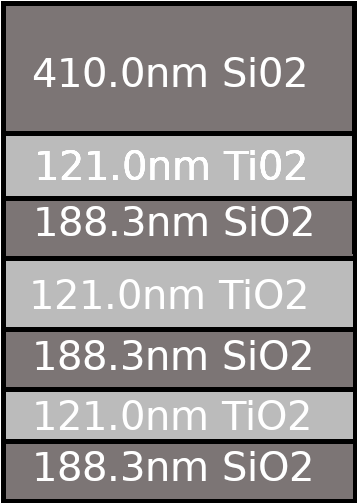
\includegraphics[width=2in]{multilayer.png}
    \caption{An illustration of the photonic crystal used in our sensor}
    \label{fig:multilayer}
\end{wrapfigure}
\hspace{0.15in}
The process of design for this experiment relies heavily on the use of a 15 milimeter right prism and our photonic crystal. The photonic crystal is composed of 3 bilayers of TiO2 and SiO2. The dielectric function of TiO2 is taken as $\epsilon_{TiO2} = 4.84 + 0.0007i$ and the dielectric function of SiO2 is taken as $\epsilon_{SiO2} = 2.1316 + 0.0001i$. 


It should be noted that the imaginary parts of each dielectric function may not be accurate and have been included to introduce some form of loss that fits the results of prior experiments. Figure 3 illustrates the structure of the multilayer.
The basic design of the sensor is split into three different parts: the primary stage, two beams, and the flowcell stage.  One of the two beams holds our laser and a focusing lens while the other holds the CCD and captures the reflected beam. Normally the laser light is too intense to pick up the surface mode in the reflected image. However, we attach a neutral density (d=3.5, see Figure \ref{fig:beams}) filter to reduce the intensity and this allows us to image the surface mode. 

% Picture of beams, central stage, and flowcell stage
\begin{figure}[h]
    \begin{center}
    \includegraphics[width=0.6\textwidth]{arms.png}
    \caption{Top: the beam holding the laser and focusing lens. Bottom: the beam holding the camera and neutral density filter.}
    \label{fig:beams}
    \end{center}
\end{figure}

Each beam is a 15cm x 10mm x 10mm aluminum MakerBeam. Attached on the left side of each beam in Figure \ref{fig:beams} is a foot used to keep the beams level with the central platform. On the right side of each beam is a 3D printed connector used to fasten the beams to the primary stage. The beams are capable of rotating around the axis that keeps these connectors in place, allowing a larger range of coupling angles for the laser-multilayer system.


The primary stage (see the green 3D printed fixture in Figure \ref{fig:centralstage}) acts as the center about which the incident beam can be coupled to the prism and then reflected onto the CCD. The design of this stage allows different types of multilayers to be used since the incident laser beam can be oriented at nearly any angle. The flowcell stage (see the blue 3D printed piece bolted into the primary stage in Figure \ref{fig:centralstage})is a modular piece that is attached to the primary stage with four bolts. The prism, multilayer, and flowcell chamber are all strapped together on this stage via 3D printed braces and hex screws. The modular nature of this piece of the sensor is very valuable since multiple designs can be used to achieve the same goal and it only takes about an hour to print off each flowcell stage. When the braces are tightened there is no liquid loss at the interface during operation, however the chamber is made of PLA and liquid will leak through the plastic after a few hours.

\begin{figure}[h]
\begin{center}
    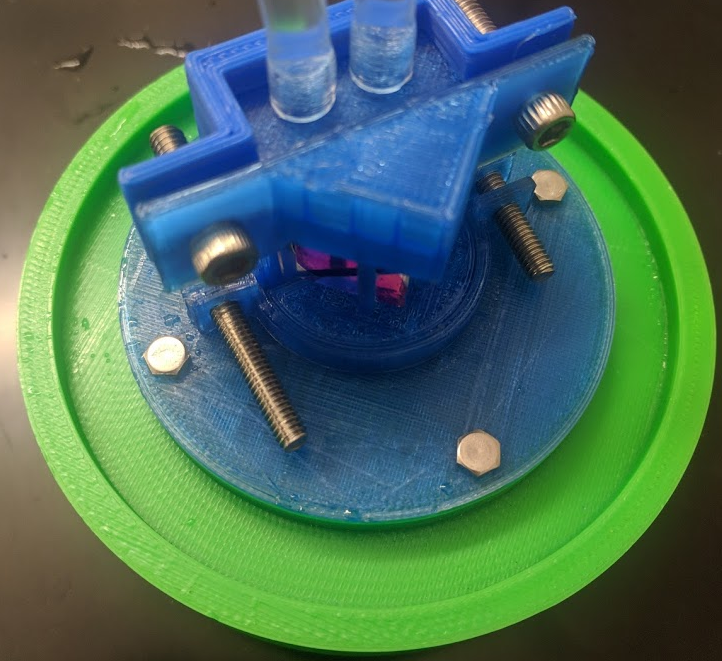
\includegraphics[width=0.6\textwidth]{central_stage.png}
    \caption{Primary stage and flowcell stage of our sensor. The green round 3D printed fixture underneath the flowcell is the primary stage which the two beams are attached to. The blue 3D printed piece mounted to the primary stage is the flowcell stage. The glass prism, multilayer, and flowcell chamber are attached atop the flowcell stage with the use of hex screws and 3D printed braces.}
    \label{fig:centralstage}
\end{center}
\end{figure}


To flow liquids through the chamber the whole fixture must be water tight. To accomplish this we designed the flowcell so that a rubber gasket could be fit around the chamber.

\begin{figure}
\begin{center}
    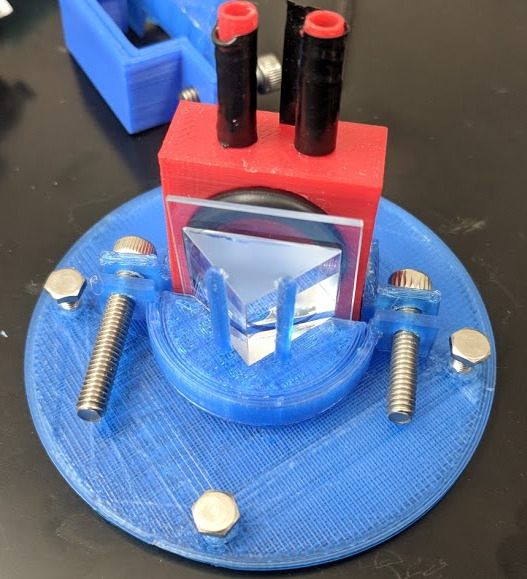
\includegraphics[width=0.6\textwidth]{flowcell.jpg}
    \caption{The flowcell stage, prism, multilayer and flowcell chamber. A rubber gasket is set in a groove around the chamber so that when the braces are tightened the interface between the multilar and flowcell is liquid tight.}
    \label{fig:flowcellstage}
\end{center}
\end{figure}
\pagebreak

% Methods
\section*{III. Methods}
\addcontentsline{toc}{section}{III.\hspace{0.12in}Methods}
\hspace{0.25in}
To collect data from our biosensor we first prepare the flowcell chamber with the correct substrate or liquid that acts as our reference point for measuring changes in optical properties. After the chamber is prepared we then turn on the beam and rotate it until the special angle is reached. 

\begin{wrapfigure}{L}{4in}
    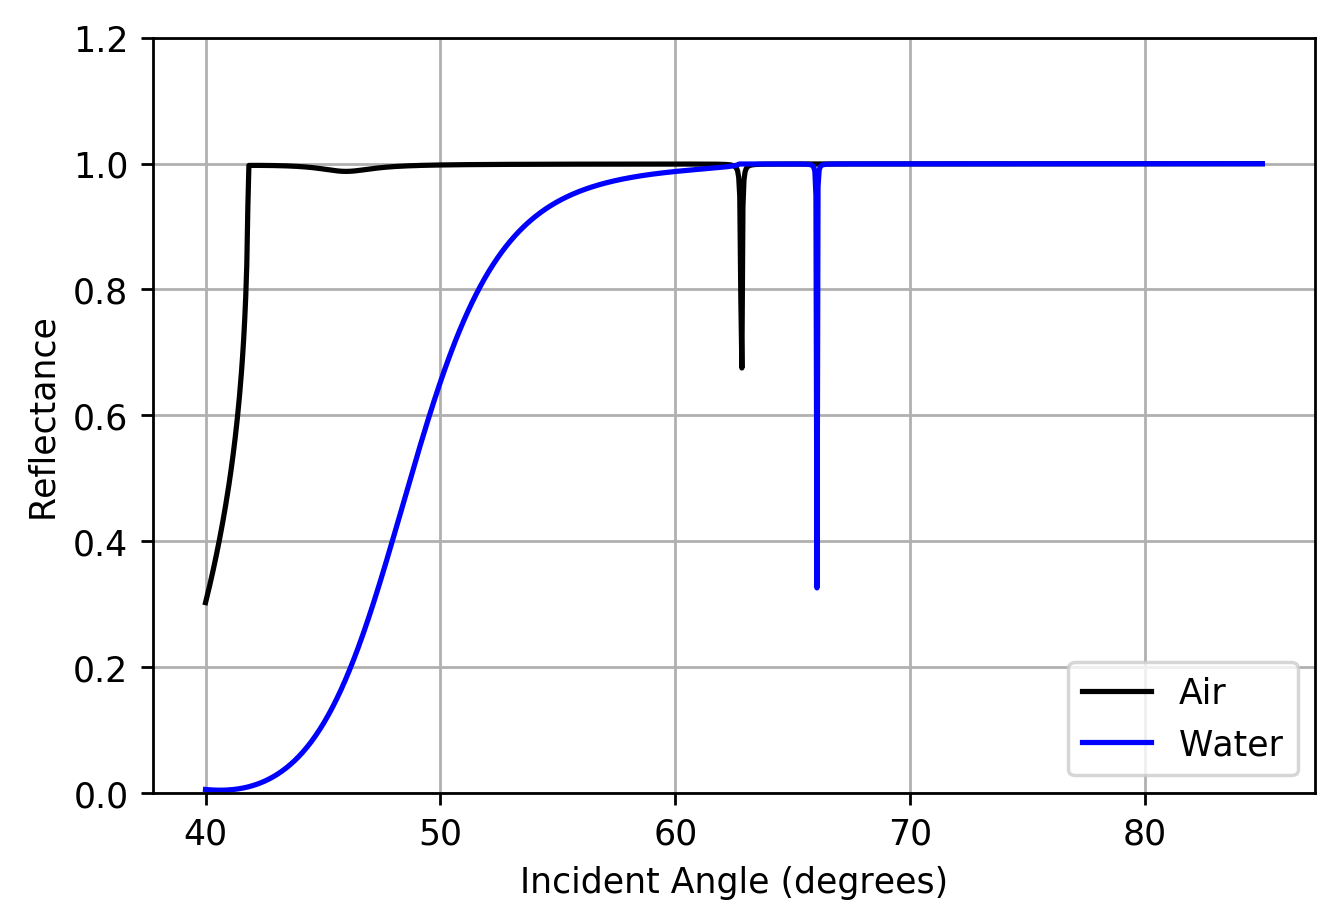
\includegraphics[width=4in]{reflectivity_dip.png}
\end{wrapfigure}

As the index of refraction inside the flowcell chamber changes the dark band will translate left or right in our reflected image, depending on whether the index is increasing or decreasing. The shift in location of the band, in pixels, corresponds to an angular shift in the part of the reflected beam giving rise to the dark band. This is shown clearly in ?? as we see that a change from an index of 1.00 (air) to 1.33 (water) corresponds to an angular shift  of about $3^\circ$.

% \begin{wrapfigure}{R}{6cm}
% 	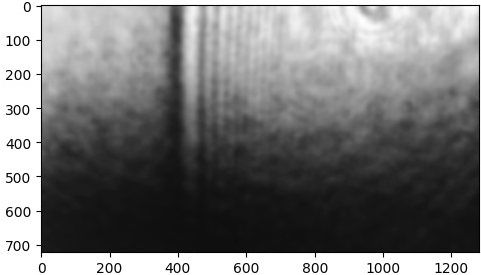
\includegraphics[width=6cm]{darkband.png}
% \end{wrapfigure}

Using the calculated data we can build a model to relate the index of refraction in the chamber to a shift in pixels on our CCD. To construct this relation we require Snell's law and some geometry. Using the classic formula for arclength and the diagram below we find:\\

\begin{figure}[h!]
\begin{center}
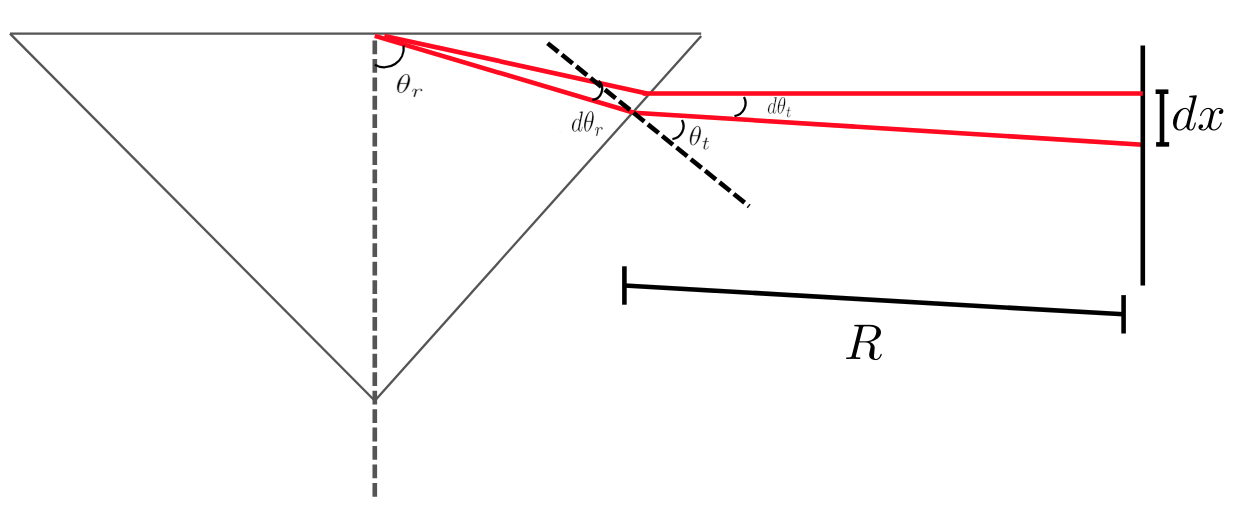
\includegraphics[width=6in]{pixelshiftfromangle.png}
\end{center}
\end{figure}

\begin{equation*}
	dx = R d\theta_t
\end{equation*}

Using Snell's law we find

\begin{equation*}
	\theta_t = \arcsin(\sin(n_g \theta_r))
\end{equation*}

Which implies that

\begin{equation*}
\begin{split}
	d\theta_t & = d\left(\arcsin\left(n_g \sin{\theta_r}\right)\right) \\
			  & = \cfrac{n_g \cos{\theta_r}}{\sqrt{1-n_g^2 \sin^{2}(\theta_r)}}\,\,d\theta_r
\end{split}
\end{equation*}


This leaves us with the relation between pixel shift and angular shift:

\begin{equation}
	dx = \cfrac{R n_g \cos{\theta_r}}{\sqrt{1-n_g^2 \sin^{2}(\theta_r)}} \,\,d\theta_r
\end{equation}

Numerically we can determine the relationship between the reflected angle and the index inside the chamber. I wrote a python program to do just that for our multilayer, assuming it is initially filled with water, and a graph of mode position ($\theta_r$) vs index of refraction is plotted below.

\begin{figure}[h]
\begin{center}
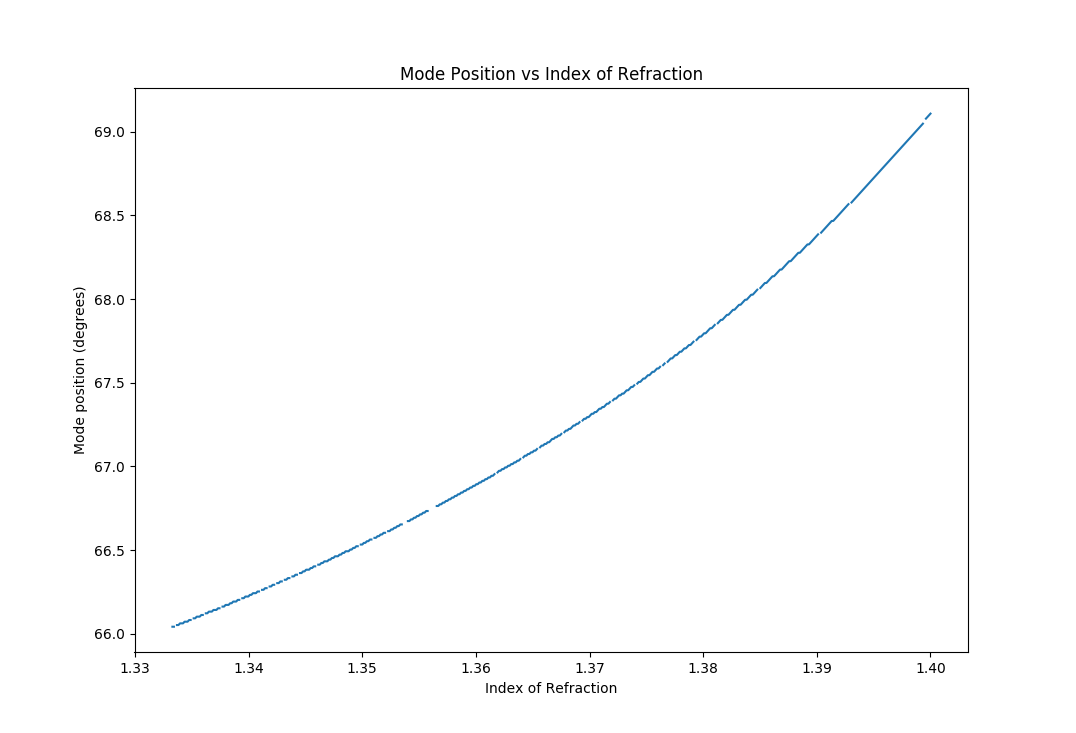
\includegraphics[width=6in]{modeposition_vs_index.png}
\end{center}
\end{figure}
\pagebreak

% Results
\section*{IV. RESULTS}
\addcontentsline{toc}{section}{IV.\hspace{0.18in}Results}
\hspace{0.25in}
The table below lists the mixtures of ethanol used to test for a change in index of refraction (*This initial data is poorly measured and more data is being taken*). The plot below shows the different indices of refraction corresponding to mixture A being injected over the interval $[45.0, 55.0]$. Similarly mixture B was injected over the interval $[60.0, 75.0]$, and mixture C over $[85.0, 95.0]$. The dip in mode position is not expected over the first two intervals as we expect the mode to shift horizontally if the index of refraction in the chamber becomes larger than the original. However, the water used had been sitting in a syringe for a few days and may have actually increased in index of refraction, meaning that the index of the water in the chamber before injecting the first mixture may have been higher than the first two mixtures.
\begin{wrapfigure}{R}{4in}
\hskip+2cm\begin{tabular}{| c c c c |}
	\hline
	Mixtures      	     &  A     & B      &  C \\
	\hline
	Ethanol (ml)  	 	 & 10.\underline{0}     & 20.\underline{0}     & 30.\underline{0} \\
	Water   (ml)  	 	 & 100.\underline{0}    & 100.\underline{0}    & 100.\underline{0} \\
   	Index         		 & 1.338\underline{0} & 1.341\underline{8} & 1.345\underline{0} \\
	\hline
\end{tabular}
	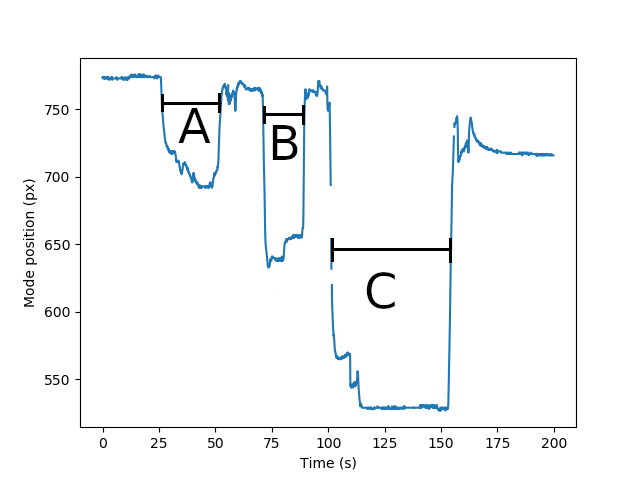
\includegraphics[width=4in]{annotated_mode_4-1-2019}
\end{wrapfigure}

\hspace{0.1in}
From this data we can infer a change in index of refraction of the medium once the index values of each mixture is known. .


\end{document}

\pagebreak

% % Conclusions

% % Bibliography
% \bibliography{references}
% \bibliographystyle{ieeetr}
% \addcontentsline{toc}{section}{References}
\end{document}